\documentclass{article}
\usepackage[T1]{fontenc}
\usepackage{lmodern}
\usepackage{graphicx}
\usepackage{amsmath,amssymb}
\usepackage[a4paper,margin=2cm]{geometry}
\usepackage[absolute,overlay]{textpos}
\setlength{\TPHorizModule}{1mm}
\setlength{\TPVertModule}{1mm}
\usepackage[indonesian]{babel}
\usepackage{hyperref}
\setlength{\emergencystretch}{2em}
% unit: Halaman 14

\begin{document}

% === Halaman 14 (python/native) ===

Empat Layanan Kriptografi

1. Kerahasiaan pesan (Confidentiality/privacy/secrecy)

2. Keaslian pesan (Data integrity)

3. Keaslian pengirim dan penerima 

      pesan (Authentication)

4. Anti penyangkalan (Non-repudiation)

14

% deskripsi: gambar native xref 84
\noindent
\includegraphics[width=0.85\textwidth]{../../images/python/page_014_img_01.png}

% deskripsi: gambar native xref 85
\noindent
\includegraphics[width=0.85\textwidth]{../../images/python/page_014_img_02.jpeg}

% deskripsi: gambar native xref 86
\noindent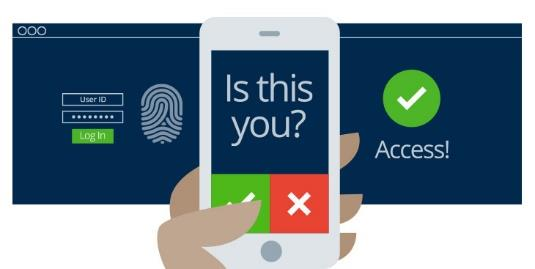
\includegraphics[width=0.85\textwidth]{../../images/python/page_014_img_03.jpeg}

% deskripsi: gambar native xref 87
\noindent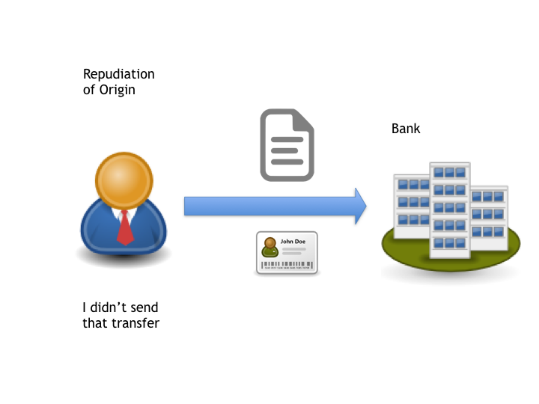
\includegraphics[width=0.85\textwidth]{../../images/python/page_014_img_04.png}

\end{document}
